\section{Key Derivation}

\subsection{Motivation}

Typically, we can generate a single source key by:

\begin{enumerate}
    \item Hardware Random Number Generator
    \item A key exchange protocol
\end{enumerate}

However, based on previous contents, there are a lot of time that we need many keys for security. So the motivation of the Key Derivation is to generate many keys from this one source key.

\subsection{Case 1: Source Key is Uniform}

Suppose Source key SK is uniform in K. We can define key derivation function (KDF) as:

\begin{equation}
    \begin{aligned}
    &\text { KDF( SK, CTX, L) := } \\
    &\qquad F(S K,(C T X \| 0))\|F(S K,(C T X \| 1))\| \cdots \| F(S K,(C T X \| L))
    \end{aligned}
\end{equation}

where CTX is a string that uniquely identifies the application. The purpose of CTX is we want get independent keys even if two apps has sampled the same SK.

\subsection{Case 2: Source Key is not Uniform}

When SK is not uniform, the PRF output may not look random. And the fact is the source key often not uniformly random.

\subsubsection{Extract-then-Expand Paradigm}

The Extract-then-Expand Paradigm has two steps:

step 1: extract pseudo-random key k from source key SK, it is shown in Figure \ref{fig: 06 Extract-then-Expland Paradigm}. where \textbf{salt} is a fixed non-secret string chosen at random.

\begin{figure}[h]
    \centering
    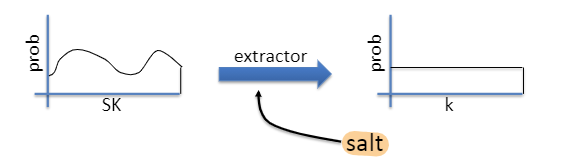
\includegraphics[width=0.5\textwidth]{Stanford_Crypto_1/fig/06_Other_Thing/Extract-then-Expland Paradigm.png}
    \caption{Extract-then-Expland Paradigm}
    \label{fig: 06 Extract-then-Expland Paradigm}
\end{figure}


step 2: expand k by using it as a PRF keys as before.


\subsubsection{HKDF: a KDF from HMAC}

Implements the extract-Then-expand paradigm:

Extract by: $\mathrm{k} \leftarrow HMAC( salt, SK)$ (salt is key, and SK is data)

Then expand using HMAC as a PRF with key $k$


\section{Deterministic Encryption}

Deterministic Encryption enables later lookup. However, attacker can tell when two ciphertexts encrypt the same message, which means we leak some information.

\subsection{Deterministic CPA Security}

The experiment of Deterministic CPA Security is shown in Figure \ref{fig: 06 Deterministic CPA Security}.

\begin{figure}[h]
    \centering
    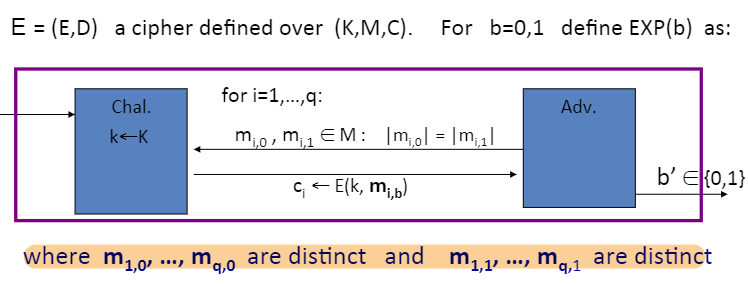
\includegraphics[width=0.5\textwidth]{Stanford_Crypto_1/fig/06_Other_Thing/Det CPA Security.png}
    \caption{Deterministic CPA Security}
    \label{fig: 06 Deterministic CPA Security}
\end{figure}

\begin{definition} [Sem Sec under det.CPA] em Sec under det.CPA

    $E$ is sem. sec. under det. CPA if for all efficient $A$ :
    $$
    \operatorname{Adv}_{\mathrm{dCPA}}[A, E]=|\operatorname{Pr}[\operatorname{EXP}(0)=1]-\operatorname{Pr}[\operatorname{EXP}(1)=1]| \quad \text { is negligible. }
    $$
    
\end{definition}

One should notice that: CBC with fixed IV is not det.CPA secure.


\section{Tweakable Encryption}



\section{Format Preserving Encryption}